Simulation codes for solving problems in mathematical physics using
mesh-based techniques continue to become increasingly sophisticated.
These codes rely on many different technological advances to help
create automated, reliable and flexible simulation tools.  For
example, technologies such as mesh generation and adaptation
contribute significantly to simulation automation and reliability.
Robust partial differential equation (PDE) discretization and error
control are central components to solution reliability.  The continued
development of more sophisticated physical models, discretizations and
coupling of physical processes in multi-physics simulations requires
software agile enough to adapt via augmentation or replacement of the
original approaches.

Traditionally, there have been four approaches used to provide
tools and technologies to simulation code developers:
\begin{enumerate}
\item complete {\it simulation codes} that support the integration of specific
      user-defined modules,
\item {\it simulation frameworks} that support the overall development process,
\item {\it libraries} that support specific aspects of the simulation
      process, and
\item {\it components} that encapsulate specific functionalities.
\end{enumerate}
The first two approaches are typified by simulation environments into
which the user inserts small customization modules.  These approaches
often require less effort on the part of the user, but provide the
least flexibility.  The latter two approaches are the opposite.  In
these cases, the users insert technologies developed by different
communities into their simulation codes and the coupling of
technologies developed by different groups can become quite
challenging.  Depending on the starting point, and needs of the
specific code development process, each approach has been found to be
useful, and we briefly describe each below.

There are many examples of complete {\it simulation codes} that
provide a small set of predefined routines that allow users to add
specific capabilities \cite{abaqus,ansys:http,fluent:http,kiva:http}.
These codes rigidly control the entire simulation information flow
with predetermined representations for the geometry, mesh and
solution.  Predefined routines allow limited access to specific
aspects of the simulation's model or discretization.  One such well
known example is ABAQUS \cite{abaqus} which supports user-defined
material and finite element routines that allow users to include their
own constitutive relationships and finite element type, respectively.
These predefined user routine interfaces place specific limits on the
functionality that can be added, but have proven useful in allowing
some customization while minimizing the development effort required by
the user.  For example, the ABAQUS material routine has been
successfully used to include hundreds of new material models ranging
from simple curve fits to complex homogenized constitutive relations
constructed from multiscale analysis.  The key disadvantages of this
approach are that the new capabilities that can be added are quite
limited, and they can only be added through a specific interface.

{\it Simulation frameworks} provide an overall structure to support
the effective development and extension of the framework to provide
new capabilities
\cite{BeSh99,overtureTR,pact93,BrLa97,De97,DoLa96,StEd04}.  Simulation
framework development efforts have taken advantage of modern
programming languages to provide users a high degree of
flexibility. However, the user must typically use predetermined data
formats, interface methods, and algorithmic and data services.  These
can vary substantially among the different frameworks, and the
differences correspond to the trade-offs associated with the types and
levels of generality supported and the computational efficiency that
can be obtained.  Frameworks can effectively manage the
information flow through simulations as long as that information
matches design decisions built into the infrastructure (e.g., one does
not attempt to use an unstructured mesh in a structured framework).
The framework approach is best suited for new simulation code
development. However, for users with an existing code who are
focused on incorporating new capabilities, the framework approach is
not ideal because integrating existing capabilities into the framework
can be a time consuming, error prone process.

The use of {\it numerical libraries} to support the development of
simulation codes has a long history. The area where numerical
libraries have been, and continue to be, most successful is for
execution of computationally intensive core numerical algorithms such
as solvers for algebraic systems, ordinary differential equations, and
differential-algebraic systems (e.g.,
\cite{AsPe98,petsc,BaGr97,eispack,lapack,linpack}). These libraries
provide capabilities that are most efficiently executed by the careful
selection and implementation of specific numerical
algorithms. Although quite successful in their specific areas,
numerical libraries do not support development of other portions of
the code.  Furthermore, integration with different functionalities
(e.g., coupling a linear solver to a discretization method) often
requires developing specific interface and coupling code for each new
library.  Hence, incorporating a new numerical library into
an existing simulation can require significant
code development and inhibits experimentation with new ideas and
methods.

Recently, application scientists have started to use {\it component
technologies} for the development of simulation codes 
\cite{keahey00ligature,ccachem,Larson:2004:CCO,mit2003,ipdps2003,norris02,SGP:Parker02,Zhou:2003:PEC}.
A {\it component} is a software object that uses a clearly defined
interface to encapsulate a specific functionality.  Components are
required to conform to a prescribed behavior which allows the object
to interact with other components via their interfaces.  Typically,
each interface is supported by multiple implementations which allows
code developers to easily experiment with different approaches.  The
use of components is ideal in the case where there is already a
substantial investment in the simulation code and the developers are
interested in incorporating advanced functionality or experimenting
with several different, related approaches.  Several groups are
developing component implementations for different aspects of the
numerical solution process including numerical solvers
\cite{petsc,BaGr97}), ODE integrators \cite{ipdps2004:odepackpp,cvode_sandia_report}, 
and visualization tools
\cite{cca-paper}.  However, more work is required to increase the
number of tools and technologies that use a component-based approach,
particularly for mesh-based simulation tools.

One of the most challenging aspects of developing a component-based
approach for mesh-based simulations is the management of the flow of
information throughout the solution process. For example, in
Figure~\ref{fig:infoFlow} we show a typical example of information
flow, starting with problem specification and domain discretization
(e.g., mesh generation).  This continues to PDE discretization and
solution.  Once the initial solution is computed, it is possible for
the information flow to return to the problem specification and domain
discretization in design optimization or adaptive mesh refinement
loops.  This information flow must be effectively managed so that data
is readily available at each stage of the solution process without the
overhead associated with data copy.

\begin{figure}
\begin{center}
%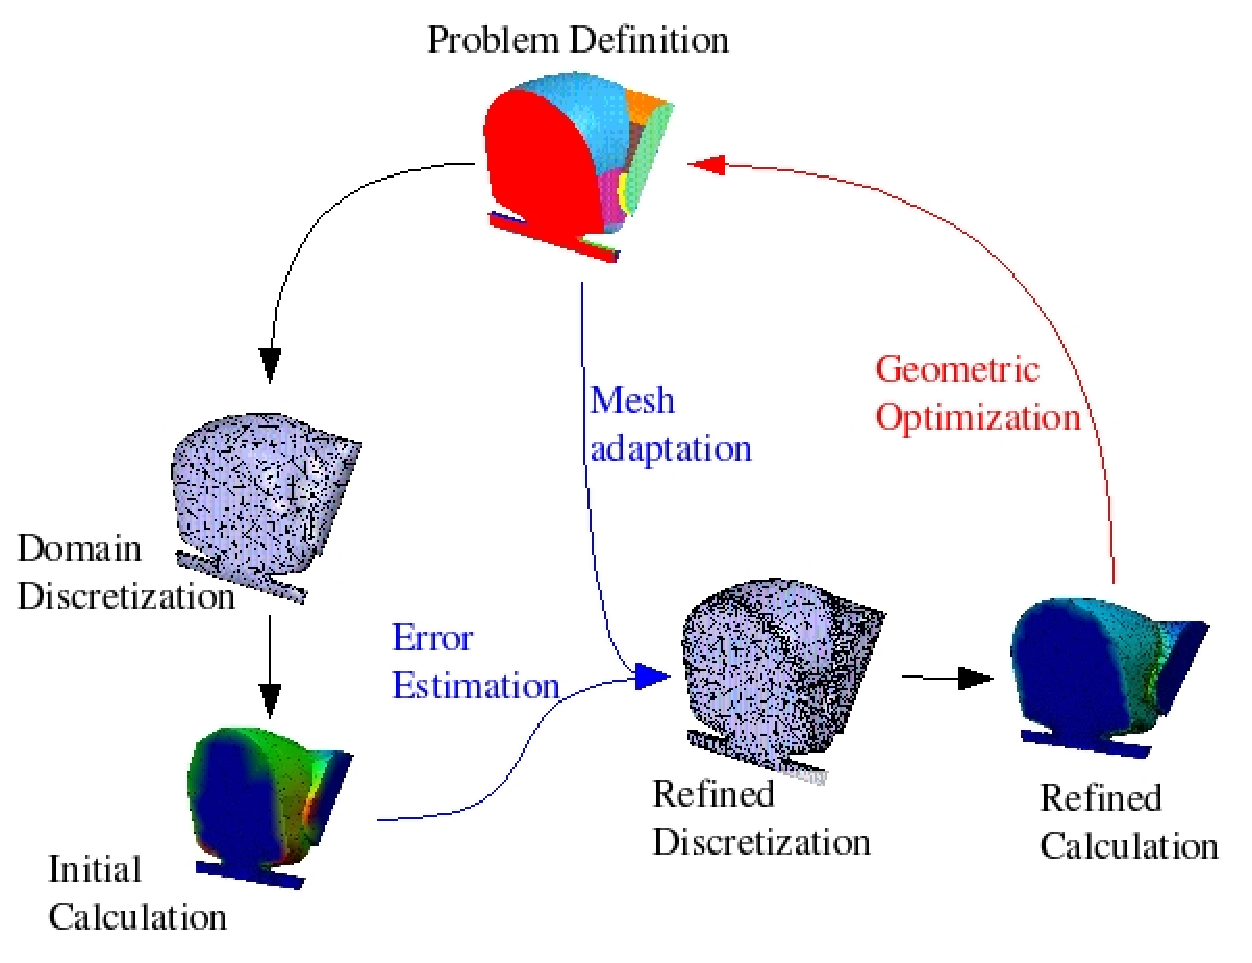
\epsfig{file=information_flow_2.eps,width=11cm}
\epsfig{file=information_flow_3.eps,width=11cm}
\caption{The information flow in a mesh-based simulation begins with
a problem definition and continues through the domain and PDE
discretizations.  Dynamic processes, such as solution adaptation and
design optimization, require components capable of feeding information
back to other parts of the information flow.}
\label{fig:infoFlow}
\end{center}
\end{figure}
 
Ongoing research in the Interoperable Tools for Advanced Petascale Simulation 
(ITAPS) Center is addressing this challenging problem by developing
geometry, mesh, and solution field components.
These three components are key conduits of the simulation information
flow and provide access to a broad set of technologies supporting
simulation automation, solution reliability and software flexibility.
Simulation automation is supported through the geometry and mesh
components because they provide ready access to CAD-based geometry
definitions and automatic mesh generators. Solution reliability is
supported because these are the components needed to support the
effective creation and adaptive control of meshes. The field and mesh
components are key to the effective coupling of multiple simulation
codes in the construction of multiscale, multiphysics simulations. 

A high level view of the information flow associated with mesh-based
simulations is presented in Section~\ref{sec:infoFlow}. This
information flow starts with a generalized problem definition and
indicates the roles of the geometry, mesh, and field components.
Section~\ref{sec:tsttdef} presents ITAPS' data model and component
specification.  In Section~\ref{sec:apps}, we illustrate the use of
ITAPS' interfaces in a number of diverse applications such as 
adaptive mesh control and mesh quality improvement.
